\documentclass[a4paper, 12pt, brazilian]{article}
\usepackage[T1]{fontenc}

\usepackage{amsmath, amsfonts, amssymb}
\usepackage{siunitx}

\usepackage[
top=2cm,
right=3cm,
bottom=2cm,
left=3cm
]{geometry}

\usepackage{xcolor}
\usepackage{tikz}
\usepackage{import}
\usepackage{float}

\usepackage{graphicx}
\usepackage{hyperref}
\usepackage{cleveref}
\usepackage{bm}
\usepackage{multirow}
\usepackage{cancel}
\usepackage[version=4]{mhchem}

\usepackage{config}

\begin{document}
	\section{Primeira questão}
	Calcule a energia fornecida pela bomba ($h_{b}$ em \SI{}{\meter}, com duas casas decimais) considerando o esquema abaixo. O aspersor localizado no ponto 2 opera com pressão de $\SI{4}{\kilogram f/\centi\meter^{2}}$ e a vazão que escoa na canalização é de $\SI{10}{\meter^{3}/\hour}$. O diâmetro da tubulação é de \SI{50}{\milli\meter} e a perda de carga total entre os pontos 1 e 2 é de \SI{15}{\meter}. A carga cinética no ponto 1 é desprezível e este ponto é uma superfície livre sujeita a pressão atmosférica. A cota em 1 vale \SI{100}{\meter} e em 2 vale \SI{146.3}{\meter}.
	\begin{center}
		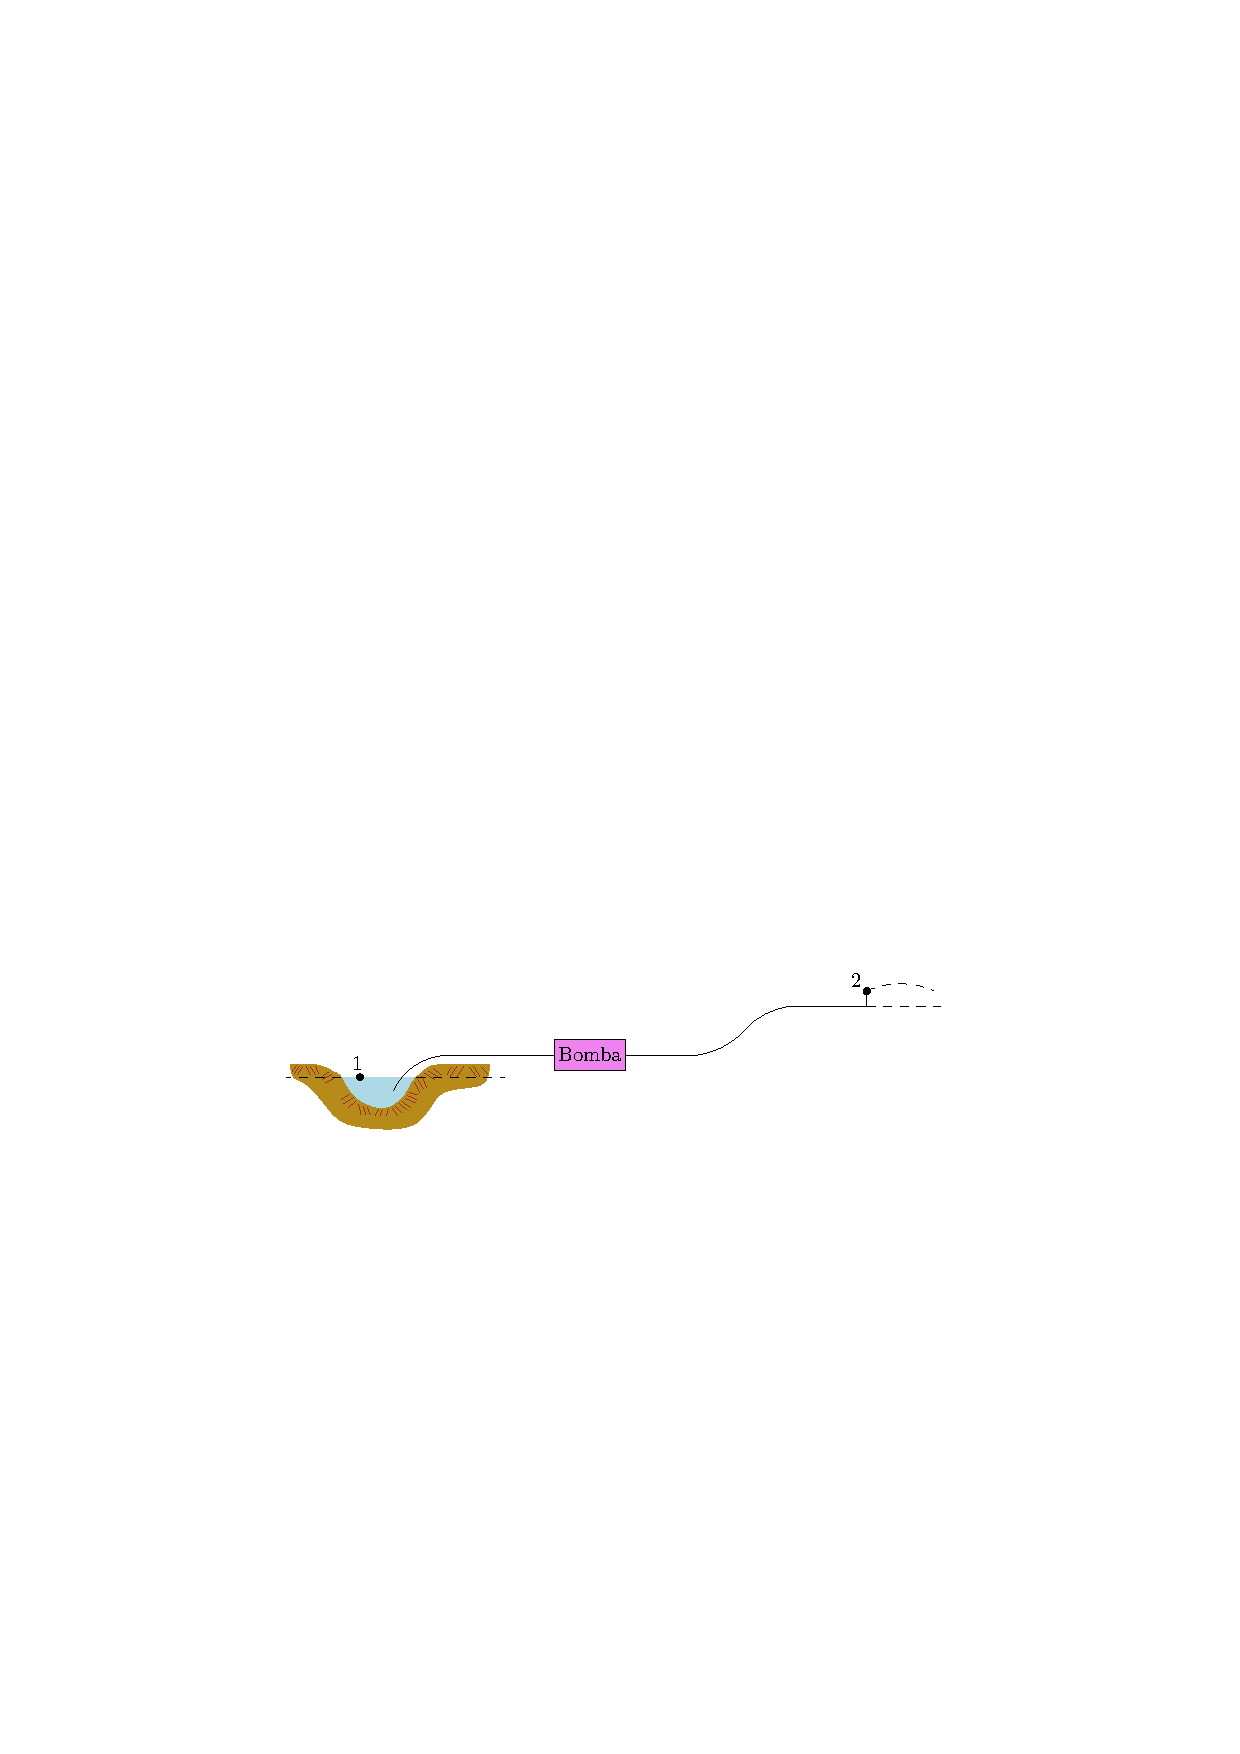
\includegraphics[width=.9\linewidth]{assets/images/ex1}
	\end{center}
	\subsection{Solução}
	A energia fornecida pela bomba pode ser dada pela equação de Bernoulli modificada como segue
	\begin{equation}
		\label{eq:bernoulli}
		Z_{1}+\dfrac{v_{1}^{2}}{2g}+\dfrac{p_{1}}{\gamma}+h_{b}=Z_{2}+\dfrac{v_{2}^{2}}{2g}+\dfrac{p_{2}}{\gamma}+hf_{1-2}
	\end{equation}
	A partir do que é dito no enunciado algumas simplificações podem ser feitas na equação anterior. Ao mudar o referencial das cotas é possível desprezar $Z_{1}$ fixando $Z_{2}=\SI{46.3}{\meter}$. No ponto 1 é cabível desprezar a pressão atuante, já que somente as moléculas da atmosfera agem. A carga cinética também é desprezada. Do lado direito da Equação de Bernoulli todos os termos serão considerados, só que para haver a substituição dos valores visando calcular $h_{b}$ as devidas conversões devem ser feitas para o Sistema Internacional.
	\begin{center}
		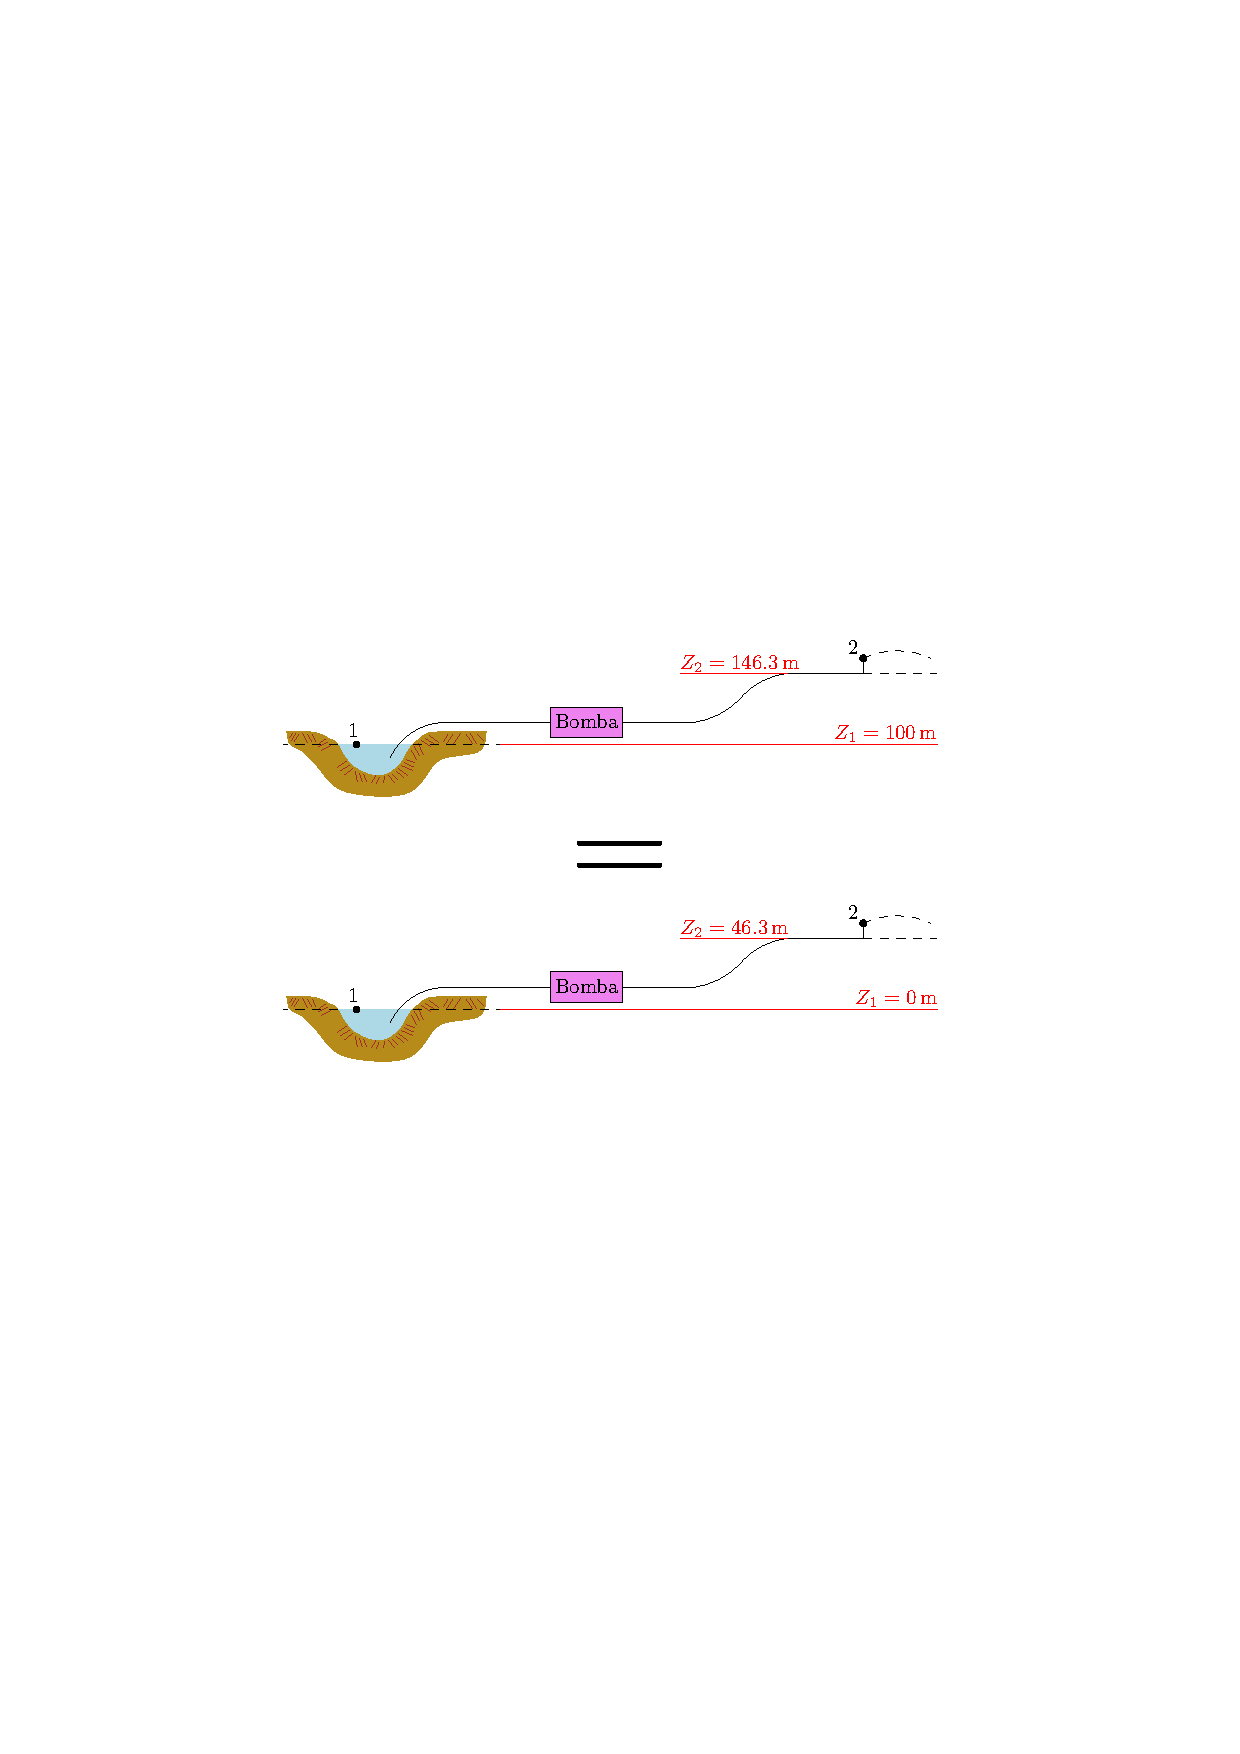
\includegraphics[width=.9\linewidth]{assets/images/referencia_1}
	\end{center}
	Para a pressão, é sabido que \SI{1}{\kilogram f} corresponde a \SI{9.81}{\newton}, então
	\begin{eqnarray}
		p_{2}&=&\SI{4}{\dfrac{\kilogram f}{\centi\meter^{2}}}\\
			 &=&\dfrac{4\cdot 9.81}{(10^{-2})^{2}}\SI{}{\dfrac{\newton}{\meter^{2}}}\\
			 &=&\SI{392400}{\pascal}
	\end{eqnarray}
	A vazão dada em $\SI{}{\meter^{3}/\hour}$ deve ser convertida para $\SI{}{\meter^{3}/\second}$ como segue
	\begin{eqnarray}
		Q_{2}&=&\SI{10}{\dfrac{\meter^{3}}{\hour}}\\
			 &=&\dfrac{10}{3600}\SI{}{\dfrac{\meter^{3}}{\second}}\\
			 &=&\SI{2.777e-3}{\meter^{3}/\second}
	\end{eqnarray}
	Após obter a vazão $Q_{2}$, para calcular a velocidade é preciso considerar a fluxo de água que atravessa a seção transversal do tubo como é descrito pela equação
	\begin{equation}
		Q_{2}=v_{2}\cdot A
	\end{equation}
	assim
	\begin{eqnarray}
		Q_{2}&=&v_{2}\cdot\dfrac{\pi\cdot d^{2}}{4}\Rightarrow\\
		\Rightarrow	v_{2}&=&\dfrac{4\cdot Q_{2}}{\pi\cdot d^{2}}
	\end{eqnarray}
	como $d_{2}=\SI{50}{\milli\meter}=\SI{.05}{\meter}$, vem
	\begin{eqnarray}
		v_{2}&=&\dfrac{4\cdot 0.0277}{\pi\cdot 0.05^{2}}\\
			 &=&\SI{1.411}{\meter/\second}
	\end{eqnarray}
	Substituindo em \eqref{eq:bernoulli}
	\begin{eqnarray}
		h_{b}&=&Z_{2}+\dfrac{v_{2}^{2}}{2g}+\dfrac{p_{2}}{\gamma}+hf_{1-2}\\
			 &=&46.3+\dfrac{1.411^{2}}{2\cdot 9.81}+\dfrac{392\,400}{9\,810}+15\\
			 &=&\SI{101.40}{\meter}
	\end{eqnarray}
\end{document}